\documentclass[UTF8, 16pt]{beamer}
 
% Chinese
\usepackage{xeCJK}

% Font
\usepackage{bookman}
\usefonttheme{serif}
% \usepackage[T1]{fontenc}
% \usepackage{tgbonum}

% Other packages
\usepackage{hyperref}
\usepackage{appendixnumberbeamer}
\usepackage{latexsym}
\usepackage{amsmath}
\usepackage{xcolor}
\usepackage{multicol}
\usepackage{booktabs}
\usepackage{graphicx}
\usepackage{listings}
\usepackage{stackengine}

% SUFE.sty
\usepackage{SUFE} 
% Bibtex
\usepackage[citestyle=authoryear-comp, 
            backend=biber, 
            bibstyle=numeric, 
%			sorting=ynt
            ]{biblatex}
\setbeamertemplate{bibliography item}[text]
\addbibresource{ref.bib}

% Other setting
\setlength{\parskip}{1em} % 设置段落之间的间距为 1em
\graphicspath{{res/}}
\setCJKmainfont{PingFang SC}
% \setCJKmonofont{Yahei Mono}

%%%%%%%%%%%%%%%%%%%%%%%%%%

% Title page
%% Author
\author[计算机协会] % The short name
{
% Name
计算机协会
% \inst{1}
% \and
% XXX 
% \inst{2}
} 
%% Title & Subtitle
\title[Java 常规教学]{Java 常规教学}
\subtitle{}
%% Institution
\institute[SUFE]
{
% \inst{1}
% Shanghai University of Finance and Economics
上海财经大学
% \and
% \inst{2}
% Shanghai University of Finance and Economics
}
%% Date
\date{23会计学院\ ACCA\ 张华轩}
%% Logo
% \logo{
\includegraphics[height=1cm]{sufe_logo}}

%%%%%%%%%%%%%%%%%%%%%%%%%%

% Document begins
\begin{document}

% Title page
\begin{frame}[noframenumbering]
    % \thispagestyle{empty}
    \titlepage{}
    % Logo
    \vspace{-0.5cm}
    \begin{figure}[htpb]
        \begin{center}
            
\includegraphics[width=0.19 \linewidth]{sufe_logo.png}
            \quad
            
\includegraphics[width=0.19 \linewidth]{ca_logo.png}
        \end{center}
    \end{figure}
\end{frame}

% Contents page
\begin{frame}{Contents}
    \tableofcontents[sectionstyle=show,
        subsectionstyle=show/shaded/hide,
        subsubsectionstyle=show/shaded/hide]
\end{frame}

% Body
% Section 1
\section{Java生态}
\begin{frame}
    \centering
    \textcolor{sufered}{Spring \& Spring Boot}
    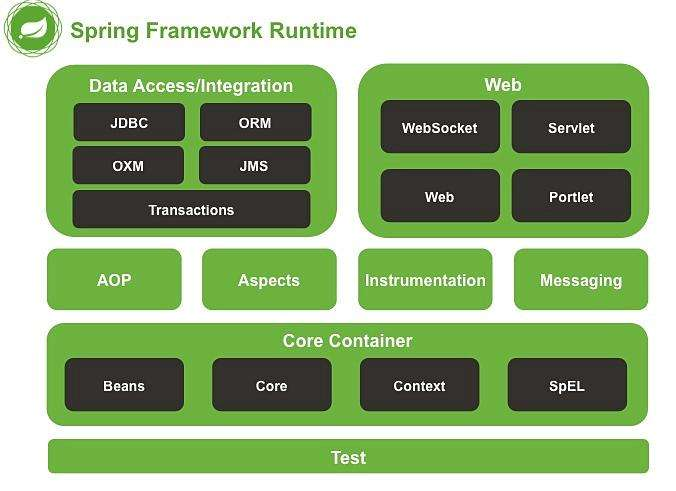
\includegraphics[width=0.95\linewidth]{ch1/spring.png}
\end{frame}

\begin{frame}
    \centering
    \textcolor{sufered}{Hadoop, Storm(Clojure), Spark(Scala)}
    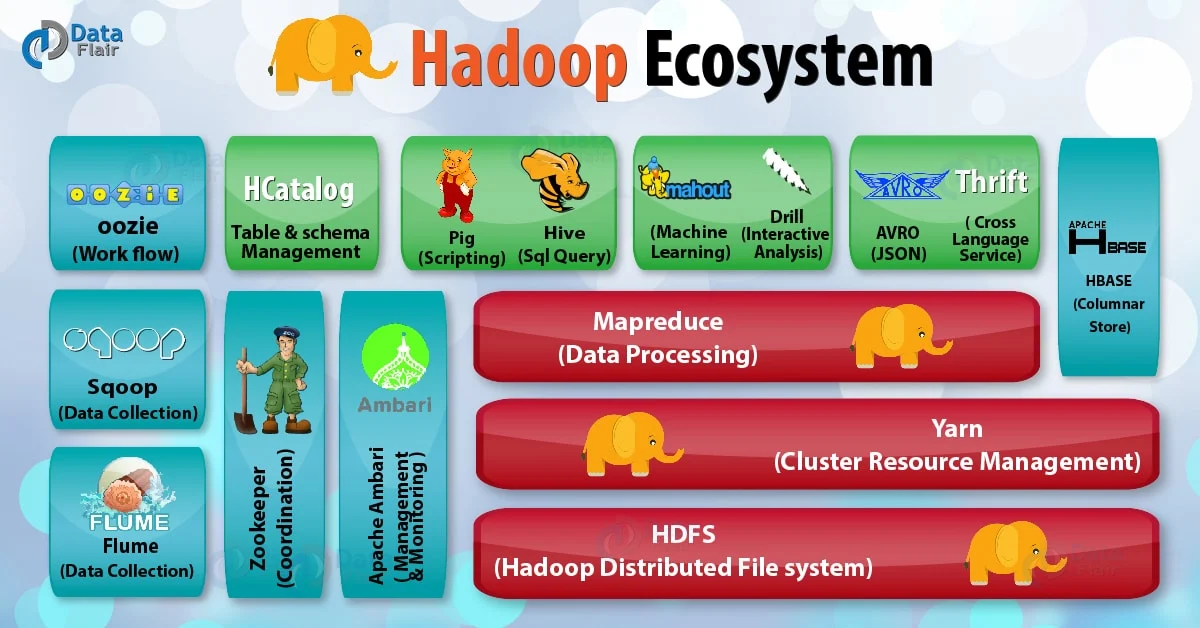
\includegraphics[width=0.95\linewidth]{ch1/hadoop.png}
\end{frame}

\begin{frame}
    \centering
    \textcolor{sufered}{Android App Development}
    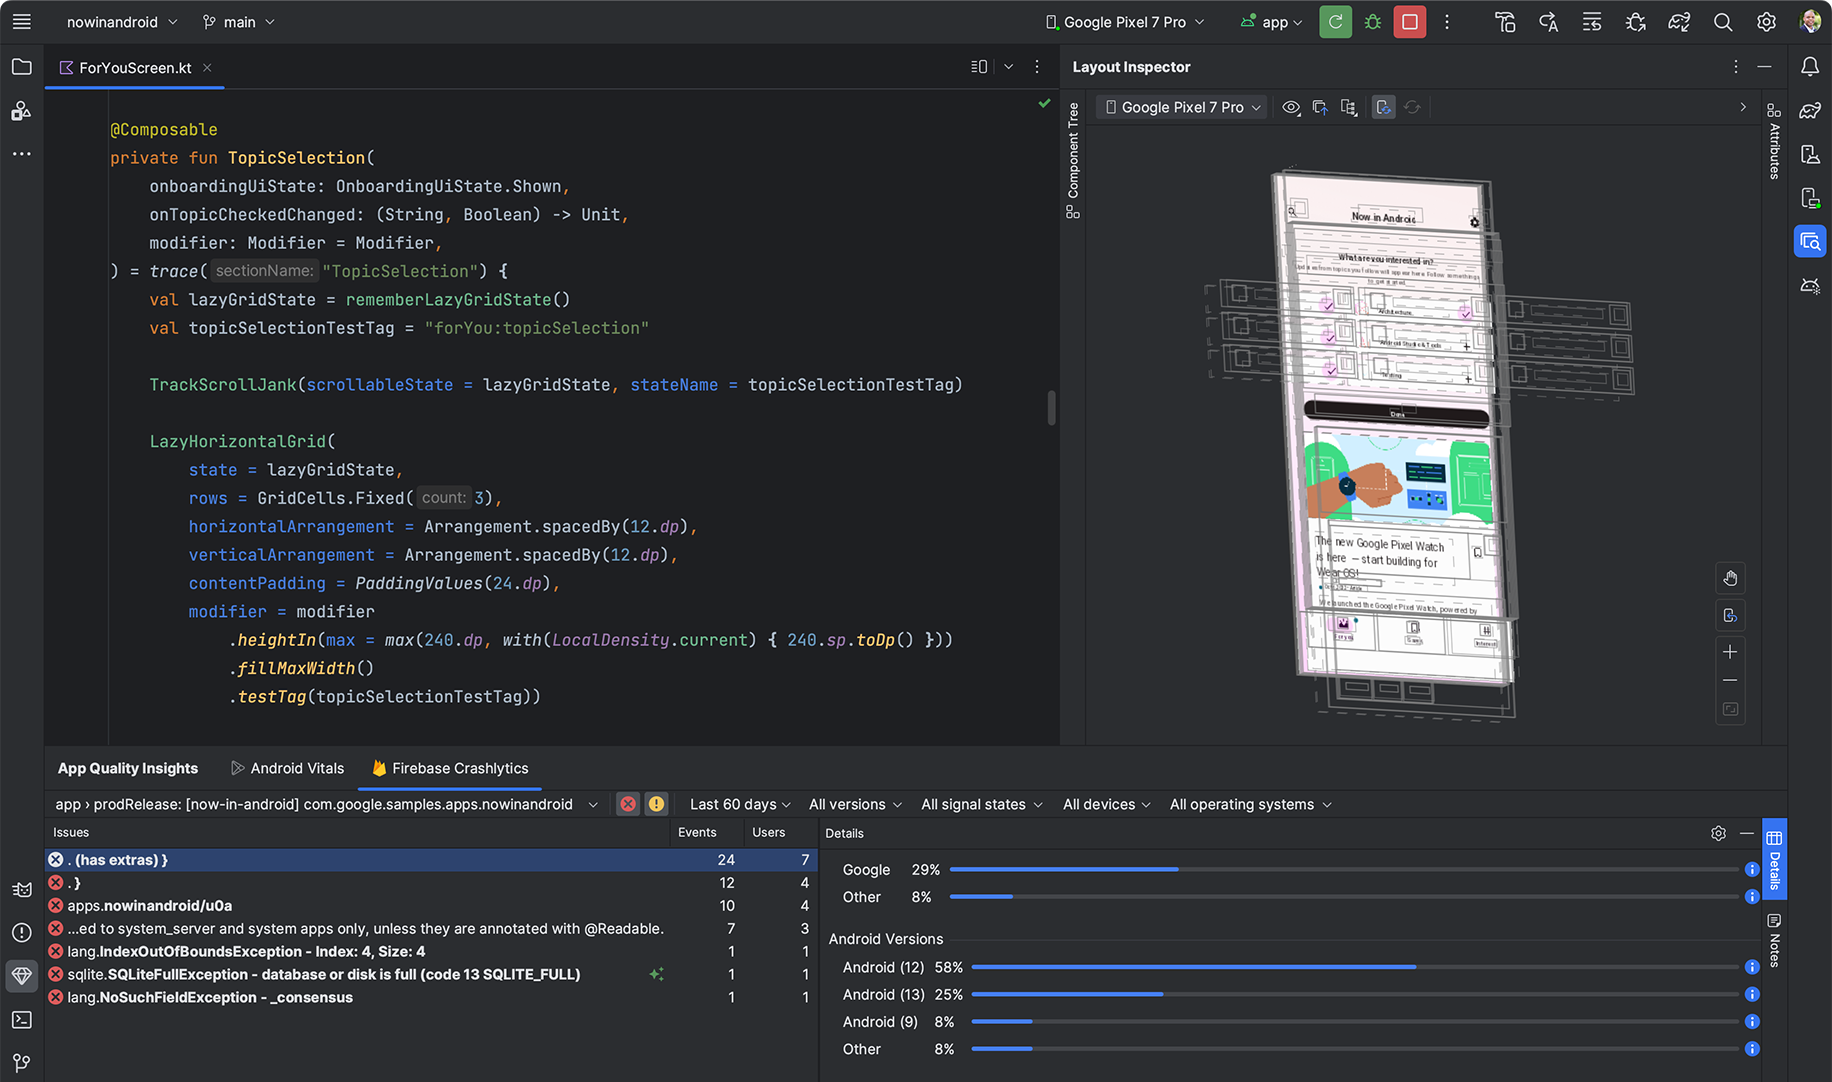
\includegraphics[width=0.95\linewidth]{ch1/as.png}
\end{frame}

% Section 2
\section{Java基础}
\begin{frame}
    \frametitle{环境配置}
    \textcolor{sufered}{?有必要吗}

    \textcolor{sufered}{谁还用命令行编译Java}

    \begin{itemize}
        \item \texttt{JRE(Java Runtime Environment)}:Java运行时环境
        \item \texttt{JDK(Java Development Kit)}:Java开发工具包
        \item \texttt{Java IDE}:Eclipse, IntelliJ IDEA, VS Code(new!)
    \end{itemize}

    \url{https://www.jetbrains.com/zh-cn/idea}

    \textcolor{sufered}{IntelliJ启动!}
\end{frame}

\begin{frame}
    \centering
    \textcolor{sufered}{Java版本演进}
    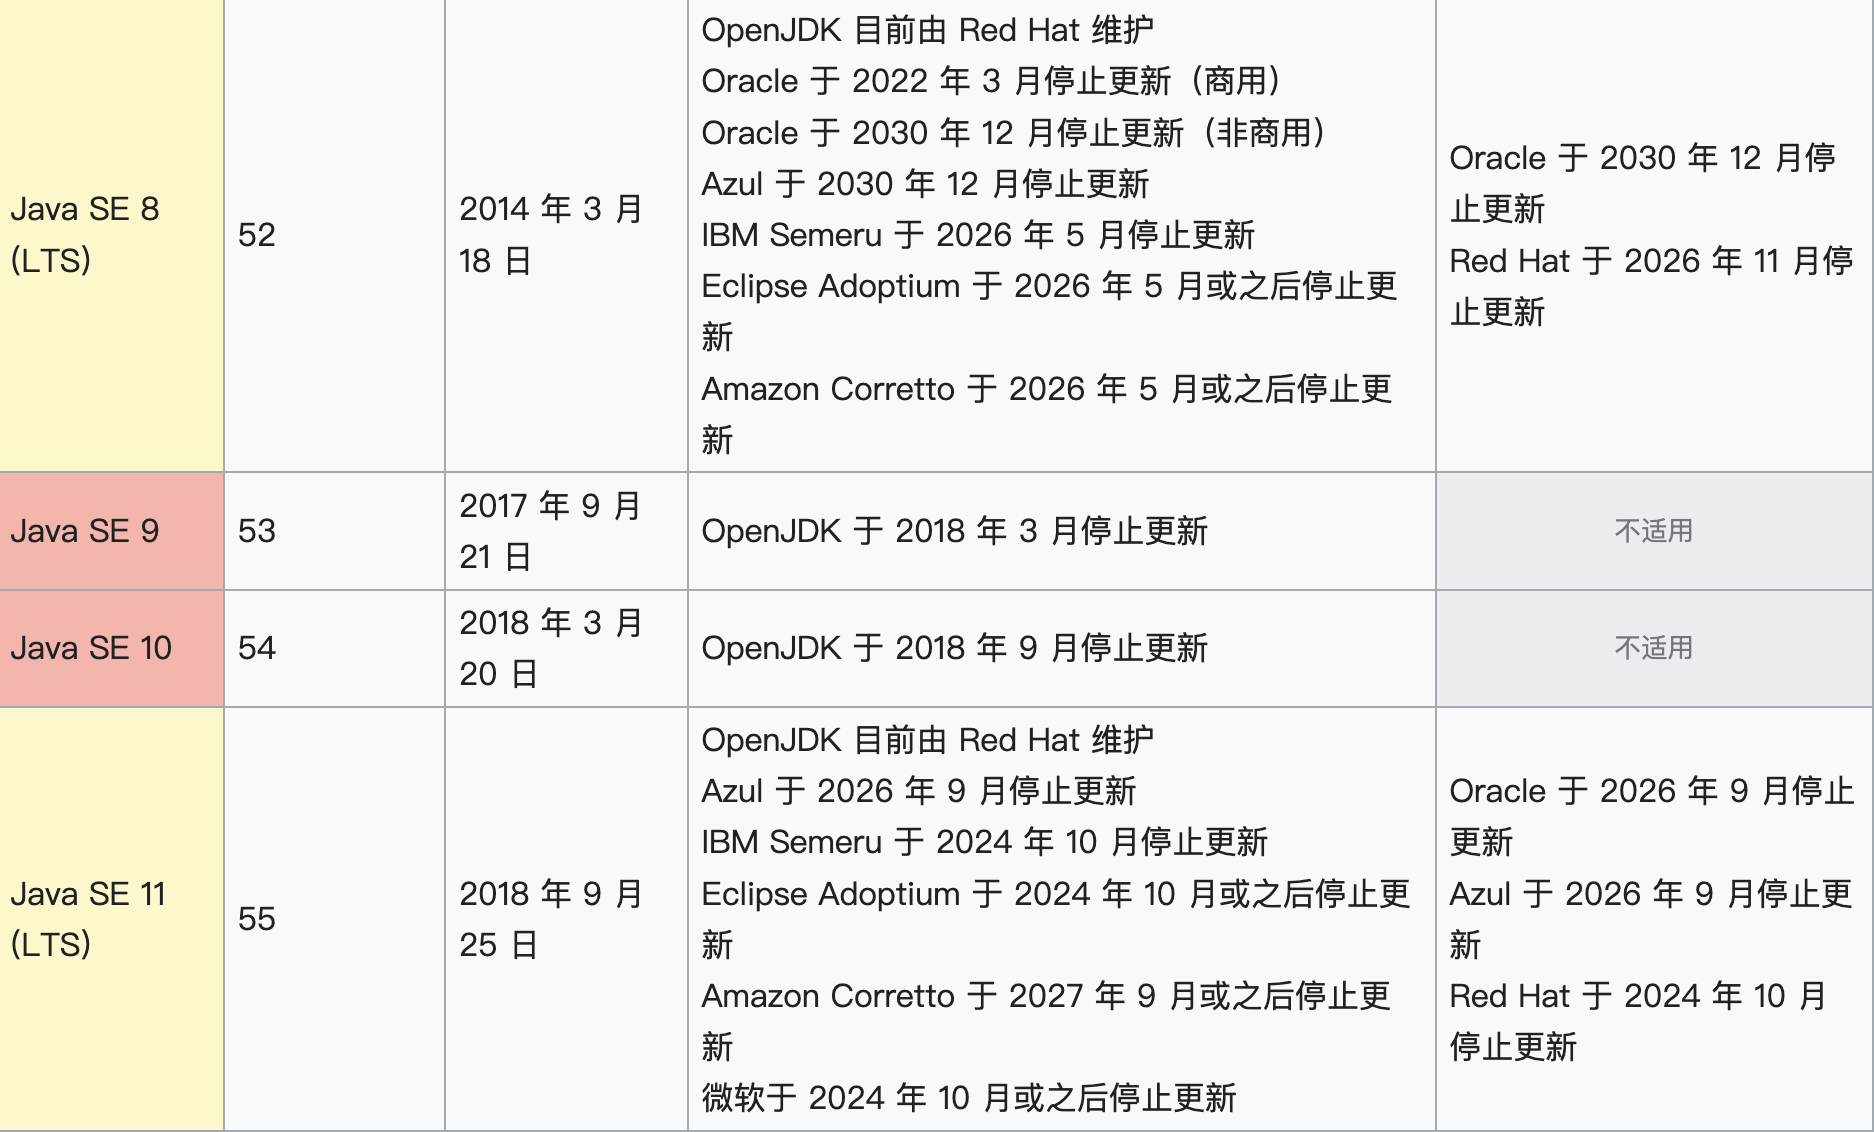
\includegraphics[width=0.95\linewidth]{ch1/edition.png}
    \texttt{Latest: Java SE 25(LTS)}
\end{frame}

\begin{frame}
    \frametitle{JDK}
    \textcolor{sufered}{主流JDK分支}

    \begin{itemize}
        \item \texttt{OpenJDK}:由社区支持、开源
        \item \texttt{Oracle JDK}:Oracle主导、商用(最后的免费商用版本是8u202)
        \item \texttt{Adoptium Eclipse Temurin}:由Eclipse基金会支持、开源
        \item \texttt{Amazon Corretto}:由Amazon主导、免费商用
    \end{itemize}

    \url{https://adoptium.net/zh-CN/temurin/releases}
\end{frame}

\begin{frame}[fragile]
    \frametitle{JVM}
    \textcolor{sufered}{Java虚拟机(Java Virtual Machine)}
    \begin{itemize}
        \item \texttt{是什么}:用于执行Java字节码的虚拟机,拥有独立的运行机制,所有Java程序都运行在JVM内部,但其运行的Java字节码未必由Java编译而成
        \item \texttt{为什么}:一次编译,到处运行;自动内存管理;自动垃圾回收功能(GC)
        \item \texttt{怎么样}:汇编->字节码,本地运行时->JVM运行时,只需要针对特定平台提供JVM实现
    \end{itemize}

    \textcolor{sufered}{JVM对内提供统一接口,对外对接本地接口}
\end{frame}

\begin{frame}
    \centering
    \textcolor{sufered}{Java虚拟机运行时}
    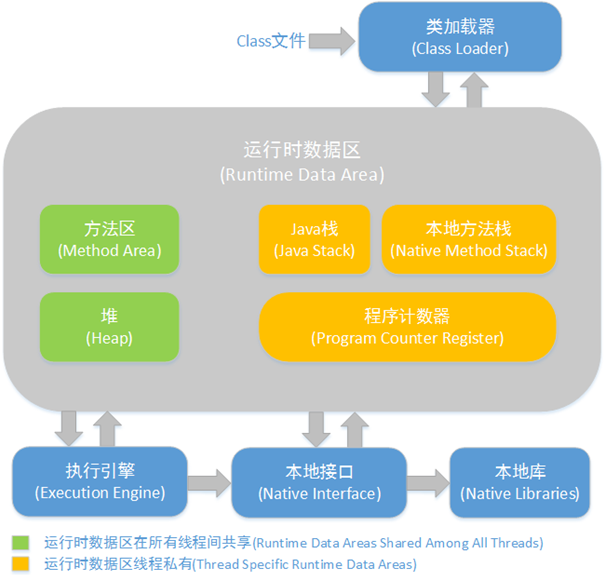
\includegraphics[width=0.75\linewidth]{ch1/jvm.jpg}
\end{frame}

\begin{frame}[fragile]
    \frametitle{基本结构}
    \textcolor{sufered}{最简单的类}
    \begin{lstlisting}
/**
* 可以用来自动创建文档的注释
**/
public class Solution {
    public static void main(String[] args) {
        // 向屏幕输出文本:
        System.out.println("Hello, world!");
        /* 多行注释开始
        注释内容
        注释结束 */
    }
} // class定义结束
    \end{lstlisting}
\end{frame}

\begin{frame}
    \frametitle{基本结构}
    \textcolor{sufered}{Annotation for Cpp}

    \begin{itemize}
        \item \textbf{入口方法}:main方法为入口方法,是程序的唯一入口
        \item \textbf{外壳类(shell class)}:Solution类在这里没有任何作用
        \item \textbf{退出码(exit code)}:main方法不返回任何值
    \end{itemize}

    \textcolor{sufered}{任何Java源文件都是类/类的集合!}
\end{frame}

\begin{frame}
    \frametitle{Dive-in}
    \textcolor{sufered}{入口方法}

    \begin{itemize}
        \item \textbf{public修饰符}:main方法是唯一的程序入口,为了让JVM可以调用,必须使用public修饰符暴露出来
        \item \textbf{static静态方法}:入口方法需要在类创建之前调用
        \item \textbf{void返回值}:JVM不接受返回值,所以返回void
    \end{itemize}
\end{frame}

\begin{frame}
    \frametitle{Java访问修饰符}
    \textcolor{sufered}{访问修饰符}

    \begin{itemize}
        \item \textbf{public}:公共访问,允许该类或成员被任何其他类访问
        \item \textbf{protected}:受保护访问,仅限于同包内的类和子类
        \item \textbf{包访问}:不加修饰符时,默认包访问,仅限同包内访问
        \item \textbf{private}:私有访问,仅限类内部访问。适用于不希望外部直接访问的属性或方法
    \end{itemize}
\end{frame}

\begin{frame}[fragile]
    \frametitle{Example}
    \textcolor{sufered}{protected子类访问}

    \begin{lstlisting}
class Parent {
    protected String message = "Hello from Parent";

    protected void displayMessage() {
        System.out.println(message);
    }
}

class Child extends Parent {
    public void show() {
        displayMessage(); // 子类可以访问父类的受保护方法
    }
}
    \end{lstlisting}
\end{frame}

\begin{frame}[fragile]
    \frametitle{Example(Continue)}
    \textcolor{sufered}{protected子类访问}
    \begin{lstlisting}
public class Main {
    public static void main(String[] args) {
        Child child = new Child();
        child.show(); // 输出: Hello from Parent
    }
}
    \end{lstlisting}
\end{frame}

\begin{frame}[fragile]
    \frametitle{Example}
    \textcolor{sufered}{protected包内访问}

    \begin{lstlisting}
package mypackage;
class Parent {
    protected String message = "Hello from Parent";

    protected void displayMessage() {
        System.out.println(message);
    }
}

class NonSubclass {
    public void accessParent() {
        Parent parent = new Parent();
        parent.displayMessage(); // 可访问包内的受保护方法
    }
}
        \end{lstlisting}
\end{frame}

\begin{frame}[fragile]
    \frametitle{Example(Continue)}
    \textcolor{sufered}{protected包内访问}

    \begin{lstlisting}
public class Main {
    public static void main(String[] args) {
        NonSubclass example = new NonSubclass();
        example.accessParent(); // 输出: Hello from Parent
    }
}
    \end{lstlisting}
\end{frame}

\begin{frame}
    \frametitle{Why protected?}
    \textcolor{sufered}{Annotation for Cpp}

    \begin{itemize}
        \item \textbf{Java}:同包内的类和子类均可以访问
        \item \textbf{C++}:仅限子类访问
    \end{itemize}

    \texttt{Java访问修饰符的设计大体参考C++}

    \textcolor{sufered}{为什么允许包内访问?}
\end{frame}

\begin{frame}[fragile]
    \frametitle{Java 包机制}
    \textcolor{sufered}{Java Package}

    \begin{itemize}
        \item \textbf{包的定义}:Java 包(Package)是一种命名空间机制,用于将相关的类和接口分组

        \item \textbf{包的作用}:
              \begin{itemize}
                  \item \textbf{命名空间}:提供独立的命名空间,防止类和接口命名冲突
                  \item \textbf{访问控制}:包允许定义类和成员的访问级别(public、protected、default和private),实现不同的封装级别。
                  \item \textbf{模块化}:将相关的类按功能分组,建立模块化的项目结构
              \end{itemize}
    \end{itemize}
\end{frame}

\begin{frame}[fragile]
    \frametitle{Example}
    \textcolor{sufered}{Java Package}
    \begin{lstlisting}
// 在 mypackage 包中定义一个类
package mypackage;

public class MyClass {
    public void display() {
        System.out.println("Hello from MyClass in mypackage");
    }
}

// 在其他类中导入该包
import mypackage.MyClass;
    \end{lstlisting}
\end{frame}

\begin{frame}
    \frametitle{设计模式:组合}
    \textcolor{sufered}{组合而非继承}

    \texttt{组合模型中,一个对象(称为复合对象)可以包含另一个对象(称为组件对象),复合对象可以使用组件对象的行为}

    \textcolor{sufered}{降低继承可能带来的耦合性}
\end{frame}

% Section 3
\section{面向对象程序设计}
\begin{frame}
    \frametitle{设计模式}
    \textcolor{sufered}{设计模式(Design Pattern)}

    是对软件设计中普遍存在(反复出现)的各种问题,所提出的解决方案
\end{frame}

\begin{frame}
    \frametitle{一题多解}
    同一输出可以由很多种程序结构来实现

    \textcolor{sufered}{设计模式要解决的问题是}
    \begin{itemize}
        \item 实用性:解决实际需求
        \item 可复用性:减少代码重复
        \item 易维护性:方便代码维护
    \end{itemize}
\end{frame}

\begin{frame}
    \frametitle{在OOP之前}
    \begin{itemize}
        \item 尼克劳斯·维尔特(Niklaus Wirth): 《算法+数据结构=程序》
        \item 传统设计模式(C-Style):结构化、过程式程序设计
    \end{itemize}

    \textcolor{sufered}{将算法放在第一位,数据结构放在第二位}
\end{frame}

\begin{frame}
    \frametitle{OOP:面向对象程序设计}
    \begin{itemize}
        \item 阿兰·凯(Alan Kay):面向对象编程的创始人之一
        \item 封装(Encapsulation):数据与操作封装在对象中
        \item 继承(Inheritance):通过继承重用代码
        \item 多态(Polymorphism):为实现同一接口的不同对象提供同一操作,产生不同行为,但该行为在逻辑上是相同的
    \end{itemize}

    \textcolor{sufered}{将对象放在第一位,强调数据与行为的结合}
\end{frame}

\begin{frame}
    \centering
    \textcolor{sufered}{Comparison Between C-Style and OOP}
    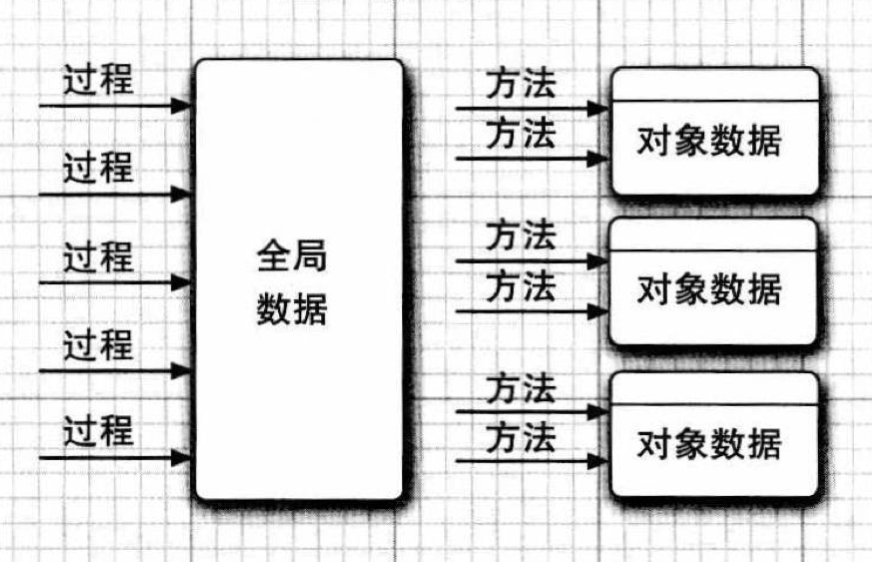
\includegraphics[width=0.95\linewidth]{ch2/oop.png}
\end{frame}

\begin{frame}
    \frametitle{对象}

    \textcolor{sufered}{对象的主要特性}
    \begin{itemize}
        \item \textbf{对象的行为 (behavior)}:可以对对象完成哪些操作,或者可以对对象应用哪些方法?
        \item \textbf{对象的状态 (state)}:当调用那些方法时,对象会如何响应?
        \item \textbf{对象的标识 (identity)}:如何区分具有相同行为与状态的不同对象?
    \end{itemize}

    \textcolor{sufered}{对象的状态与标识是每个对象独有的,即便在同一类的实例中,也存在差异}
\end{frame}

\begin{frame}
    \frametitle{一些术语}

    \begin{itemize}
        \item \textbf{行为 $\approx$ 方法}
        \item \textbf{状态 $\approx$ 属性 $\approx$ 字段}
    \end{itemize}
    \textcolor{sufered}{相对来讲,行为和状态更为抽象}

    方法、属性和字段通常可以特指,而行为和状态则可以理解为是它们的集合
\end{frame}

\begin{frame}
    \frametitle{Example}
    \begin{table}
        \centering
        \vspace{-0.5cm}
        \setlength{\tabcolsep}{5mm}
        {
            \begin{tabular}{lcc}
                \toprule %\hline
                \textbf{现实世界} & \textbf{计算机模型} & \textbf{Java代码}                      \\ \midrule
                人             & 类 / class      & \texttt{class Person \{ \}}          \\
                小明            & 实例 / ming      & \texttt{Person ming = new Person();} \\
                小红            & 实例 / hong      & \texttt{Person hong = new Person();} \\
                小军            & 实例 / jun       & \texttt{Person jun = new Person();}  \\ \bottomrule
            \end{tabular}
        }
    \end{table}
\end{frame}

\begin{frame}[fragile]
    \frametitle{Example(Continue)}
    \textcolor{sufered}{Person类及其实例}
    \begin{lstlisting}
class Person {
    public String name;
    public int age;
}

Person ming = new Person();
ming.name = "Xiao Ming"; // 对字段name赋值
ming.age = 12; // 对字段age赋值
System.out.println(ming.name); // 访问字段name

Person hong = new Person();
hong.name = "Xiao Hong";
hong.age = 15;
    \end{lstlisting}
\end{frame}

\begin{frame}
    \centering
    \textcolor{sufered}{Person类及其实例}
    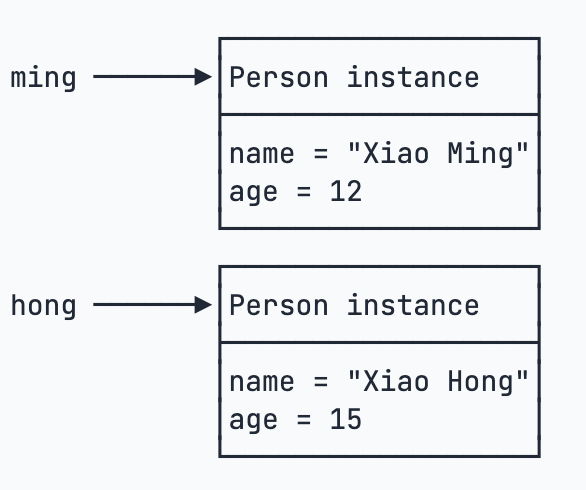
\includegraphics[width=0.8\linewidth]{ch2/person.png}
\end{frame}

\begin{frame}[fragile]
    \frametitle{封装性}
    \textcolor{sufered}{public带来的逻辑混乱}
    \begin{lstlisting}
Person ming = new Person();
ming.name = "Xiao Ming";
ming.age = -99; // age设置为负数 
    \end{lstlisting}
\end{frame}

\begin{frame}[fragile]
    \frametitle{封装性}
    \textcolor{sufered}{试试private?}
    \begin{lstlisting}
public class Main {
    public static void main(String[] args) {
        Person ming = new Person();
        ming.name = "Xiao Ming"; // 对字段name赋值
        ming.age = 12; // 对字段age赋值
        // Error: not visible!!!
    }
}

class Person {
    private String name;
    private int age;
}
    \end{lstlisting}
\end{frame}

\begin{frame}
    \frametitle{this变量}
    \textcolor{sufered}{回忆}

    前面我们在外部代码中使用形似ming.name的语法修改ming实例的字段

    如何在类的内部代码中修改当前实例的字段?
\end{frame}

\begin{frame}
    \frametitle{this变量(Continue)}
    \textcolor{sufered}{变量this是方法内部的隐含变量,它始终指向当前实例}
\end{frame}

\begin{frame}[fragile]
    \frametitle{方法}
    \textcolor{sufered}{方法允许外部代码间接修改对象状态}
    \begin{lstlisting}
class Person {
    private String name;
    private int age;
        
    public String getName() {
        return this.name;
    }
        
    public void setName(String name) {
        this.name = name;
    }
    ...
}
    \end{lstlisting}
\end{frame}

\begin{frame}[fragile]
    \frametitle{方法(Continue)}
    \begin{lstlisting}
class Person {
    ...
    public int getAge() {
        return this.age;
    }
    
    public void setAge(int age) {
        if (age < 0 || age > 100) {
            throw new IllegalArgumentException();
        }
        this.age = age;
    }
}
    \end{lstlisting}
\end{frame}

\begin{frame}[fragile]
    \frametitle{方法(Continue)}
    \textcolor{sufered}{现在我们可以通过方法来修改对象属性}
    \begin{lstlisting}
public class Main {
    public static void main(String[] args) {
        Person ming = new Person();
        ming.setName("Xiao Ming"); // 设置name
        ming.setAge(12); // 设置age
        System.out.println(ming.getName() + ", " + ming.getAge());
    }
}
    \end{lstlisting}
\end{frame}

\begin{frame}
    \frametitle{封装}
    \textcolor{sufered}{封装(Encapsulation)}

    是面向对象编程的核心特性之一,它指的是将对象的状态与行为封装在一起,对外部只暴露必要的接口
\end{frame}

\begin{frame}
    \frametitle{为什么封装?}

    \begin{enumerate}
        \item \textbf{隐藏内部实现}:
              外部无法直接访问和修改对象的内部数据,只能通过对象提供的方法进行操作,可减少错误和不当使用

        \item \textbf{增强安全性和可靠性}:
              封装性确保对象的内部状态不会因外部干扰而处于不一致的状态

        \item \textbf{易于维护和扩展}:
              封装可以更改对象的内部实现而不影响使用对象的代码,从而提高代码的灵活性和可维护性

        \item \textbf{提高代码的模块化}:
              封装使得每个对象可以被视为一个独立的模块,便于开发者更好地理解和管理复杂的系统
    \end{enumerate}
\end{frame}

% End
\begin{frame}[allowframebreaks]%{End}
    \begin{center}
        \Huge\textbf{\textit{\texttt{Thanks!}}}
    \end{center}
\end{frame}

% Reference
\appendix
\begin{frame}{Reference}
    \nocite{corejava}
    \nocite{liaoxuefeng}
    \addtocounter{framenumber}{-1}
    \printbibliography{} % [heading=bibintoc, title=Reference]
\end{frame}

\end{document}